% !TEX encoding = UTF-8 Unicode

%%%%%%%%%%%%%%%%%%%% author.tex %%%%%%%%%%%%%%%%%%%%%%%%%%%%%%%%%%%
%
% sample root file for your "contribution" to a proceedings volume
%
% Use this file as a template for your own input.
%
%%%%%%%%%%%%%%%% Springer %%%%%%%%%%%%%%%%%%%%%%%%%%%%%%%%%%


\documentclass[conference]{IEEEtran}
%
% RECOMMENDED %%%%%%%%%%%%%%%%%%%%%%%%%%%%%%%%%%%%%%%%%%%%%%%%%%%
%

% to typeset URLs, URIs, and DOIs
% https://www.overleaf.com/learn/latex/Hyperlinks
\usepackage{hyperref}
\hypersetup{
    colorlinks=true,
    linkcolor=blue,
    filecolor=magenta,      
    urlcolor=cyan,
    pdftitle={Overleaf Example},
    pdfpagemode=FullScreen,
    }

\def\UrlFont{\rmfamily}

\usepackage[T1]{fontenc}
\usepackage[utf8]{inputenc}
\usepackage[textsize=scriptsize]{todonotes}
\usepackage{gensymb}
\usepackage{array,multirow}
\usepackage{caption} 
\usepackage{subcaption}
\captionsetup[table]{skip=10pt}
\usepackage{makecell}

\usepackage{cite}
\usepackage{amsmath,amssymb,amsfonts}
\usepackage{bm}
\usepackage{algorithmic}
\usepackage{graphicx}
\usepackage{textcomp}
\usepackage{xcolor}
\def\BibTeX{{\rm B\kern-.05em{\sc i\kern-.025em b}\kern-.08em
    T\kern-.1667em\lower.7ex\hbox{E}\kern-.125emX}}

\usepackage{graphicx}
\graphicspath{ {./img/} }

\renewcommand{\labelenumii}{\theenumii}
\renewcommand{\theenumii}{\theenumi.\arabic{enumii}.}

\begin{document}
%
\title{Zastosowanie regulatora PID i CNN do sterowania robotem Duckiebot}
% \title{Application of PID and CNN controllers to control the Duckiebot robot}


\author{
\IEEEauthorblockN{1\textsuperscript{st} Marek Długosz}
\IEEEauthorblockA{\textit{AGH University of Science and Technology}\\
Cracow, Poland \\
mdlugosz@agh.edu.pl \\
0000-0001-6827-9149}\\[0.4cm]
\IEEEauthorblockN{3\textsuperscript{rd} Marcin Szelest}
\IEEEauthorblockA{\textit{IEEE Senior Member}}
\IEEEauthorblockA{\textit{AGH University of Science and Technology} \\
Cracow, Poland \\
mszelest@agh.edu.pl\\
0000-0002-0522-1270}
\and
\IEEEauthorblockN{2\textsuperscript{nd} Paweł Skruch}
\IEEEauthorblockA{\textit{IEEE Senior Member}}
\IEEEauthorblockA{\textit{AGH University of Science and Technology} \\
Cracow, Poland \\
pawel.skruch@agh.edu.pl\\
0000-0002-8290-8375}\\
\IEEEauthorblockN{4\textsuperscript{th} Artur Morys-Magiera}
\IEEEauthorblockA{\textit{AGH University of Science and Technology} \\
Cracow, Poland \\
amorys@student.agh.edu.pl\\
0000-0002-2137-8841}
}


\maketitle              % typeset the title of the contribution

\begin{abstract}
W artykule przedstawiono projekt i praktyczną realizację przez studentów układu sterowania
z wykorzystaniem klasycznego regulatora PID i regulatora wykorzystującego sztuczne sieci neurnowe.
Obiektem sterowania jest robot Duckiebot a zadanie jakie ma realizować polega na jeździe robota wzdłuż wyznaczonej lini (\emph{linie follower}). Celem proponowanych aktywności jest zapoznanie studentów z zaletami  i wadami obydwu użytych regulatorów oraz nabycia przez nich umiejętności praktycznej realizacji układów sterowania. 
W artykule krótko opisano sposób działania obydwu regulatorów, sposób ich praktycznej implementacji oraz opisano w jaki sposób praktycznie należy zrealizować ćwiczenie. 
\end{abstract}


% We would like to encourage you to list your keywords within
% the abstract section using the \keywords{...} command.
\begin{IEEEkeywords}
% autonomouse robot, PID controller, convolutional neural network, line follower
autonomiczny robot, regulator PID, konwolucyjne sieci neuronowe, line follower
\end{IEEEkeywords}
%
\section{Introduction}
Ostatnimi latami można zaobserwować swoisty renesans w wykorzystaniu sztucznych sieci neuronowych. Powstały i są ogólnie dostępne różnego rodzaju architektury sieci, udoskonalono ich metody trenowania. Wszystko to sprawiło, że  sztuczne sieci neuronowe są coraz częściej, z sukcesem, wykorzystywane w układach automatycznego sterowania \cite{algor2030973, 786109}. Zastosowanie sieci neuronowych w układach automatyki nie jest ich typowym wykorzystaniem ponieważ bardzo często sterowanie może być realizowane z wykorzystaniem dobrze znanych i opisanych klasycznych algorytmów sterowania (PID, LQR, MPC itp.). Daje to okazję do porównania działa dwóch różnych technologii, znalezienia ich wad oraz plusów. W procesie kształcenia studentów projekt i wykonanie przez nich układu sterowania z wykorzystaniem klasycznych algorytmów sterowania oraz sztucznych sieci neuronowych jest bardzo interesujące zarówno z punktu naukowego jak i dydaktycznego.

Istotnym elementem kształcenia studentów podnoszącym atrakcyjność samych zajęć, dającym możliwość rozwiązywania problemów praktycznych jest wykorzystanie rzeczywistych robotów. Jednym z takich projektów dostarczających kompletną platformę robotyczną (sprzęt, oprogramowanie, symulator, materiały dydaktyczne) jest projekt Duckietown.
Projekt Duckietown powstał w 2016 na uniwersytecie Massachusetts Institute of Technology (MIT) w ramach zajęć dla studentów \cite{paull2017duckietown}. Jest to otwarty projekt, którego celem jest promowanie edukacji i badań związanych z autonomią robotów, zwłaszcza w kontekście samochodów autonomicznych. W ramach projektu, powstały roboty Duckiebot, makiety miast Duckietown po których poruszają się roboty, oraz dodatkowa infrastrukturę, taką jak np. Watchtower, wspomagającą proces nawigacji. 
Projekt obejmuje także stworzenie oprogramowania symulacyjnego o nazwie Duckiebot-GYM, które umożliwia symulację pracy robotów w wirtualnym środowisku \cite{gym_duckietown}. Obecnie dostępna jest już druga generacja robotów Duckiebot, w której do sterowania wykorzystuje się komputer Jetson Nano. Wykorzystanie platformy Jetson Nano otwiera drzwi do wykorzystania zaawansowanych sieci neuronowych z dedykowanym wsparciem GPU do sterowania robotem Duckiebot.

Artykuł zorganizowany jest następująco, w sekcji \ref{sec:problem-definition} zdefiniowano problem do rozwiązania, w sekcji \ref{sec:student-activity} opisano aktywności studentów realizowane w trakcie rozwiązywania  problemu. Sekcja \ref{sec:robot-duckiebot} zawiera krótki projektu Duckietown oraz konstrukcji i sposobu sterowania robotem Duckiebot, w sekcjach \ref{sec:pid-controller} i \ref{sec:nn-controller} opisano sposób rozwiązania problemu z wykorzystaniem regulatora PID i regulatora wykorzystującego sztuczne sieci neuronowe. W sekcji \ref{sec:practical-info} podano kilka praktycznych wskazówek pomocnych w trakcie realizacji zadania i w ostaniej sekcji \ref{sec:conclusion} zawarto wnioski.

%%%%%%%%%%%%%%%%%%%%%%%%%%%%%%%%%%%%%%%%%%%%%%%%%%%%

\section{Definicja problemu}\label{sec:problem-definition}
Ramach procesu dydaktycznego, studenci mają za cel zaprojektować układ automatycznego sterowania robotem o napędzie różnicowym który realizuje funkcjonalność poruszania się po wyznaczonej trasie. Trasa robota oznaczona jest linią o kolorze (np. kolor czerwony, żółty itp.) różnym od podłoża (najczęściej w kolorze czarnym) po którym porusza się robot. Kształt trasy stanowi zamknięty kontur. Układ sterowania powinien generować sygnał sterowania aby minimalizować całkowity błąd odchyłki robota od zadanej trasy.  Tego typu zadanie, jest typowym zdaniem implementowanym w różnego rodzaju robotach autonomicznych i często jest określane jako \emph{line follower}.  

%%%%%%%%%%%%%%%%%%%%%%%%%%%%%%%%%%%%%%%%%%%%%%%%%%%%

\section{Studenckie aktywności}\label{sec:student-activity}
W ramach zdefiniowanego problemu w sekcji \ref{sec:problem-definition} studenci będą musieli się wykazać odpowiednim przygotowaniem teoretycznym oraz umiejętnościami praktycznymi takimi jak: 
znajomość zasady działania regulatora PID, znajomość zasady działania sztucznych sieci neuronowych, znajomość operacji związanych z przekształceniami obrazów, umiejętność implementacji regulatora PID w wersji dyskretnej, umiejętność implementacji wybranych struktur sieci neuronowych, umiejętność implementowania operacji przekształceń obrazów, znajomość zagadnień związanych z doborem parametrów regulatora PID, znajomość zagadnień związanych z uczeniem sieci neuronowych i przygotowaniem danych do ich uczenia, ocena poprawności procesu uczenia sieci. Z pozoru prosty algorytm sterowania nieskomplikowanym robotem realizujący funkcjonalność \emph{line follower} generuje szereg zadań których wykonanie wymaga odpowiedniego przygotowania teoretycznego jak i praktycznego studentów. Należy również zauważyć, że problemy które studenci muszą rozwiązać w trakcie realizacji projektu są typowymi problemami które występują w przy programowaniu innego typu robotów autonomicznych.

%%%%%%%%%%%%%%%%%%%%%%%%%%%%%%%%%%%%%%%%%%%%%%%%%%%%

\section{Robot Duckiebot}\label{sec:robot-duckiebot}
Robot Duckiebot jest niewielkim, dwu kołowym robotem zdolnym do poruszania się po płaskich nawierzchniach. Do napędu robota wykorzystano dwa moduły zawierające: silnik elektryczny, przekładnię i enkoder. Robot Duckiebot wyposażony jest w następujące sensory: kamera RGB, czujnik odległości oraz czujnik bezwładnościowy IMU \cite{gupta2022low}. Do sterowanie robotem wykorzystany jest komputer JetsonNANO. Dodatkowo robot Duckiebot wyposażony jest w cztery diody RGB które mogą być wykorzystany np. do sygnalizowania stanu w jakim aktualnie znajduje się robot. Robot Duckiebot jest zaprojektowany do autonomicznego sterowania i może poruszać się bez udziału człowieka, na podstawie danych z kamery i odpowiednich algorytmów sterowania. Na rysunku\;\ref{fig:duckiebot-3d} przedstawiono robota Duckiebot w trzech rzutach.

\begin{figure}[h]
    \centering
    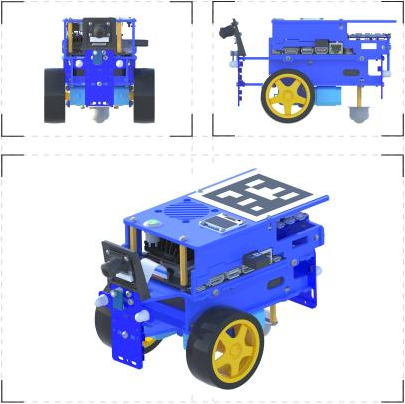
\includegraphics[width=.9\columnwidth]{duckiebot-blue-3d}
    \caption{Robot Duckiebot (\url{http://duckietown.org}).}
    \label{fig:duckiebot-3d}
\end{figure}

Konsekwencją zastosowania dwóch niezależnych silników elektryczny w konstrukcji robota Duckiebot jest sposób w jaki kontroluje się kierunek poruszania się robota.
Robot Duckiebot wykonuje zakręty zmieniając prędkości obrotowe silników elektrycznych w zależności od tego w jaką stronę chce zakręcić oraz jak duży ma być promień skrętu.
Do sterowania robotem wykorzystywane są dwa sygnały: $v$-wartość prędkości liniowej oraz $\omega$-wartość prędkości obrotowej wzdłuż osi pionowej Z robota, zob. rys. \ref{fig:duckiebot-kinematics}.

\begin{figure}[h]
    \centering
    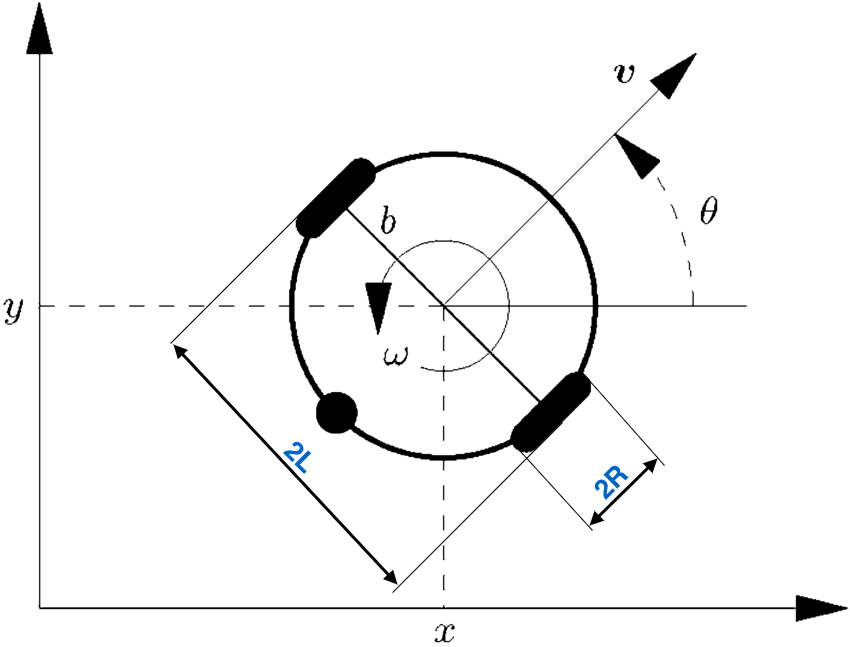
\includegraphics[width=.8\columnwidth]{dt-kinematic}
    \caption{Układ kinematyczny robota Duckiebot.}
    \label{fig:duckiebot-kinematics}
\end{figure}

Znając wartości $(v, \omega)$ (wyznaczone np. przez regulator) możemy obliczyć prędkości obrotowe kół robota z wzorów \eqref{eq:omega-L} i \eqref{eq:omega-R}:

\begin{eqnarray}
	\omega_L & = & \cfrac{v-L\omega}{R} \label{eq:omega-L} \\
	\omega_R & = & \cfrac{v+L\omega}{R} \label{eq:omega-R}
\end{eqnarray}
\\
Tego typu układ sterowania robotem Duckiebot jest bardzo często wykorzystywany w robotyce i nosi nazwę \emph{differential drive robot} \cite{siegwart2011introduction}. Zaletą takiego układu kinematycznego ruch robota Duckiebot jest prostota konstrukcji (brak mechanizmów osi skrętnych kół) natomiast wadą jest konieczność ciągłego kontrolowania prędkości obrotowej kół robota ($\omega_R$, $\omega_L$) tak aby poruszał się on po zadanej trasie.

%%%%%%%%%%%%%%%%%%%%%%%%%%%%%%%%%%%%%%%%%%%%%%%%%%%%

\section{Klasyczna realizacja z regulatorem PID}\label{sec:pid-controller}
Klasyczny układu sterowania robotem Duckiebot wykorzystuje regulator PID. Zadniem układu sterowania jest generowanie takiego sygnału sterowania $u_i$ aby minimalizować wartość sygnału błędu $e_i$, gdzie $i$-kolejne chwile czasowe. Na rysunku \ref{fig:pid-pipeline} przedstawiona schemat blokowy układu sterowania robotem Duckiebot z wykorzystaniem regulatora PID oraz kamery robota jako sensorem.

\begin{figure}[h]
    \centering
    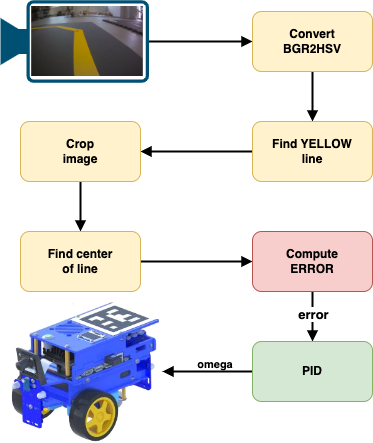
\includegraphics[width=.8\columnwidth]{PipeLinePID}
    \caption{Schemat układu sterowania robotem Duckiebot z wykorzystaniem regulatora PID.}
    \label{fig:pid-pipeline}
\end{figure}

Sygnał błędu $e_i$ zdefiniowany jest jako różnica pomiędzy środkiem osi pionowej obrazu z kamery a punktem znajdującym się w analizowanym obszarze obrazu zawierającym linię wzdłuż której powinien poruszać się robot Duckiebot, zob. rys.\;\ref{fig:error-definition}. 

\begin{figure}[h]
    \centering
    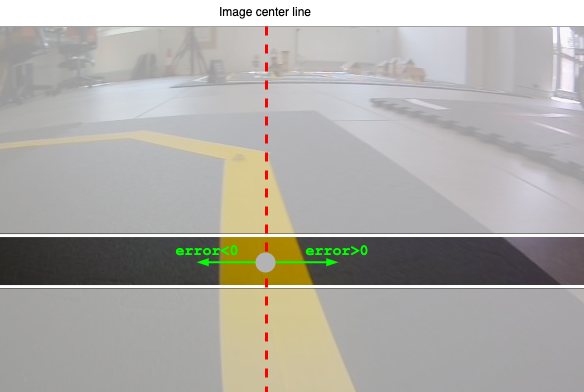
\includegraphics[width=.95\columnwidth]{ErrorDefinition.png}
    \caption{Określenie błędu dla układu sterowania realizującego funkcjonalność \emph{line follower} dla robota Duckiebot.}
    \label{fig:error-definition}
\end{figure}

Układ sterowania robota Duckiebot jest systemem dyskretnym (zaimplementowanym na komputerze JetsoNANO) dlatego należy wykorzystać wersję dyskretną regulatora PID. Uwzględniając rodzaj napędu robot Duckiebot (napęd różnicowy \emph{differential drive robot}) sygnał sterowania $u_i$ wygenerowany przez regulatora PID odpowiada prędkości obrotowej $\omega_i$ wzdłuż osi Z robota.

\subsection{Regulator PID}
Jednym z najlepiej poznanych i najczęściej stosowanych regulatorów w układach automatycznego sterowania jest regulator PID. Wynika to przede wszystkim z jego uniwersalności, łatwości realizacji zarówno w formie analogowej jak i cyfrowej oraz w miarę prostego i intuicyjnego sposobu strojenia parametrów regulatora PID. Regulator PID w wersji dyskretnej który zastosowano w układzie sterowania robotem Duckietown dany jest równaniem:

\begin{equation}
u_i = K_p e_i + K_i \sum_{i=0}^k{e_i \Delta t} + K_d \cfrac{e_i-e_{i-1}}{\Delta t}
\label{eq:pid-dis}
\end{equation}
%https://github.com/duckietown/mooc-exercises/blob/c476a67fea9836beab99eed23cfc1a83c77af7bb/modcon/solution/05-PID-Control/PID_controller.ipynb
gdzie: $K_p$ wzmocnienie części proporcjonalnej, $K_i$ wzmocnienie części całkującej, $K_d$ wzmocnienie części różniczkującej, $e_i$ błąd w $i$-tej chwili czasu, $\Delta t$ krok czasowy \cite{aastrom2021feedback}.

\subsection{Pomiar błędu}
Wartość sygnału błędu $e_i$ wyznaczana jest na podstawie obrazów przesyłanych przez kamerę robota Duckiebot. W celu określenia wartości sygnału $e_i$ konieczne jest wykonanie kilku operacji na przesłanych obrazach (zob. rys. \ref{fig:pid-pipeline}). 
Pierwszym operacją jest konwersja obrazu z przestrzeni barw RGB to przestrzeni HSV (\emph{Hue}, \emph{Saturation}, \emph{Value}). Takie przekształcenie przestrzeni barw obrazów ma na celu przede wszystkim lepsze rozróżnianie i rozpoznawanie kolorów. 
Kolejną operacją jest znalezienie na obrazie lini o określonym kolorze wzdłuż której ma poruszać się robot Duckiebot. Taka operacja ma na celu pozostawienia na obrazie tylko lini wyznaczającej trasę robotą i usunięcie z obrazu wszystkich pozostałych elementów (np. tło). 
Kolejna operacją jest ograniczenie obszaru analizowanego poprzez wykonanie operacji przycięcia. Operacja ta ma na celu dokładne znalezienie środka lini wzdłuż której ma poruszać się robot Duckiebot. 
Środek lini znajdywany jest jako współrzędne środka ciężkości otrzymanego, w wyniku poprzednich przekształceń, lini wyznaczającej trasę robota Duckiebot. Na rysunku \ref{fig:img-transformation-summary} pokazano rezultat poszczególnych przekształceń wykonywanych na obraza z kamery robota w celu wyznaczenia wartości błędu położenia $e_i$.

\begin{figure}[hbt!]
    \centering
    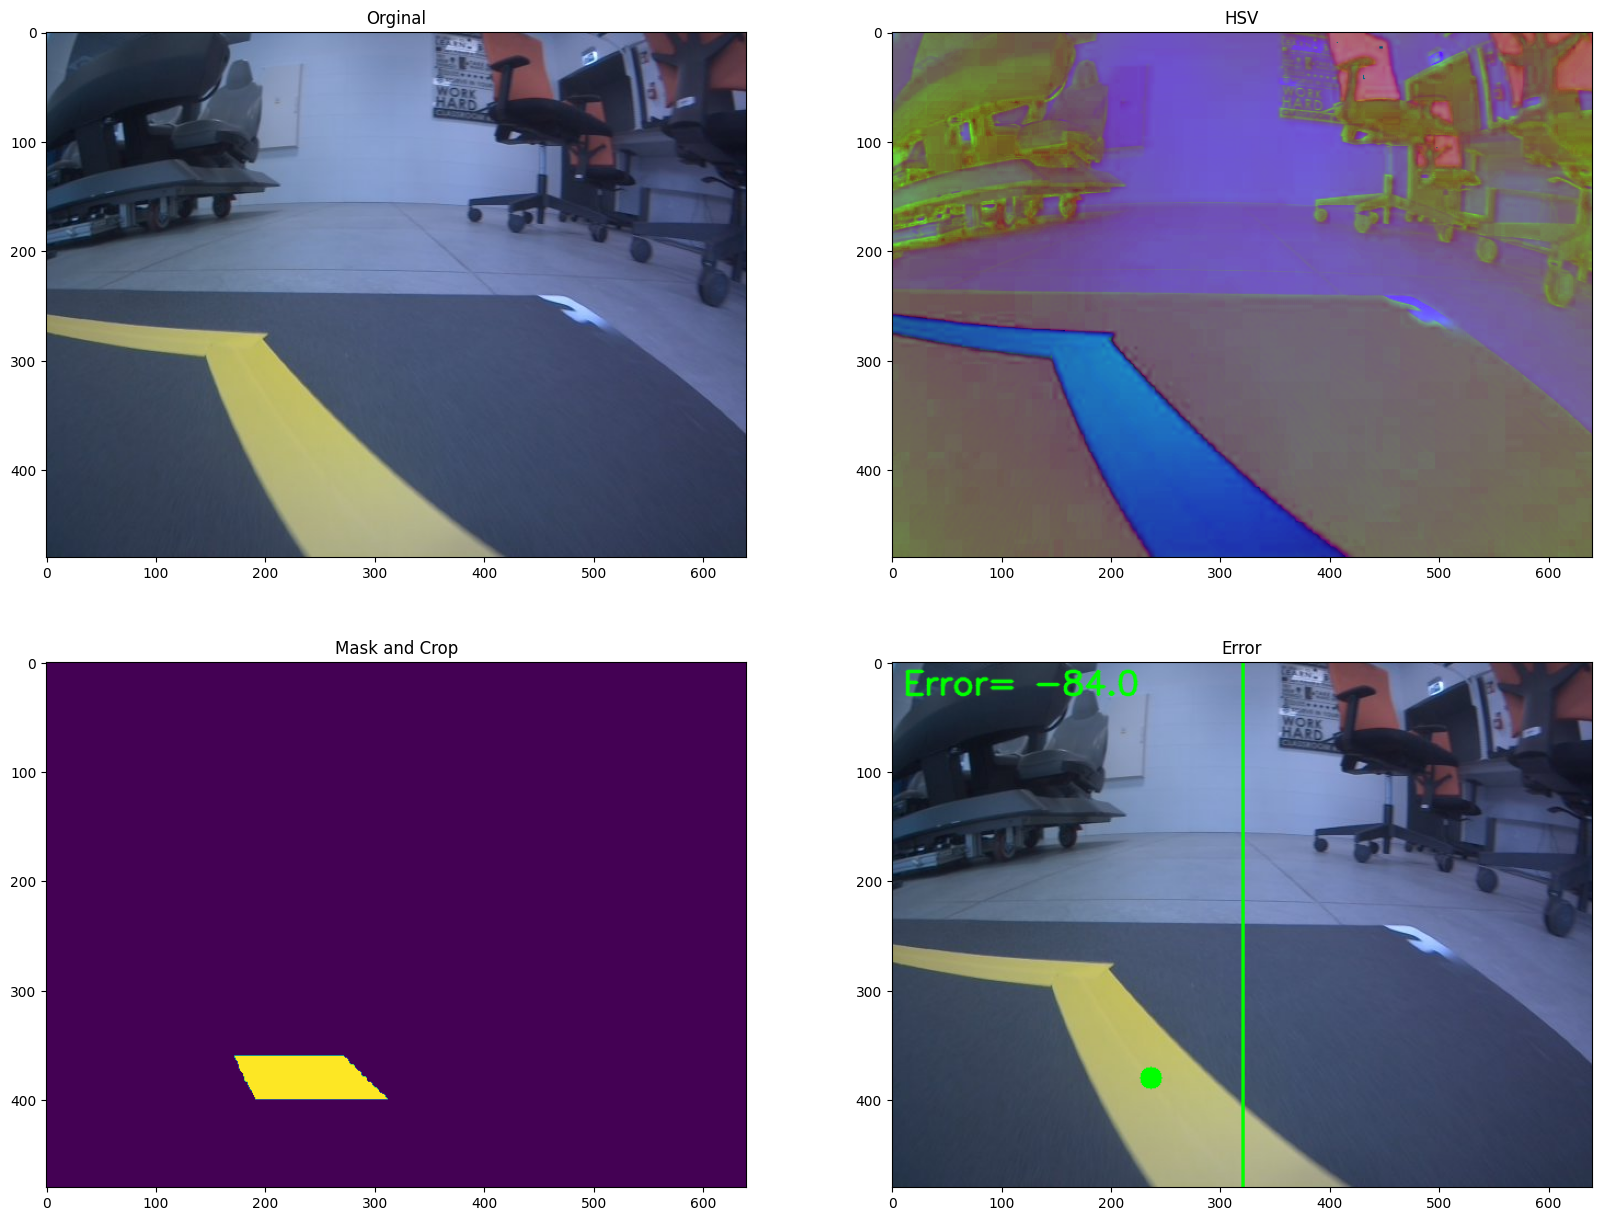
\includegraphics[width=.95\columnwidth]{img-transformation.png}
    \caption{Operacje wykonywane na obrazach z kamery robota w celu wyznaczenie błędu położenia $e_i$.}
    \label{fig:img-transformation-summary}
\end{figure}

Na końcu wartości błędu położenia $e_i$ jest normalizowana do przedziału $e_i \in [-1;\;1]$. Ma to na celu uniezależnieniu się od rozmiarów (szerokość, wysokość) obrazów przesyłanych z kamery.

%%%%%%%%%%%%%%%%%%%%%%%%%%%%%%%%%%%%%%%%%%%%%%%%%%%%

\section{Realizacja z wykorzystaniem sieci neuronowych}\label{sec:nn-controller}
Drugi ze sposobów generowania sygnału sterowania $u_i$ wykorzystuje konwolucyjną sieć neurnową (\emph{Convolutional Neural Network} CNN). Schemat blokowy układu regulacji wykorzystującego sieci neuronowe przedstawiono na rys. \ref{fig:cnn-pipeline}.

\begin{figure}[h]
    \centering
    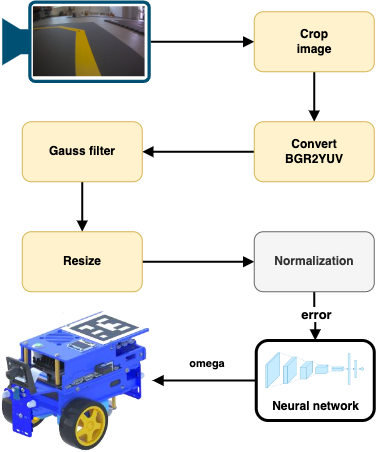
\includegraphics[width=.8\columnwidth]{NNPipeline3}
    \caption{Schemat układu sterowania robotem Duckiebot z wykorzystaniem konwolucyjnych sieci neurnowych.}
    \label{fig:cnn-pipeline}
\end{figure}

Konwolucyjne sieci neuronowe są bardzo skuteczne szczególnie w zadaniach rozpoznawania wzorców i przetwarzania obrazów. Sieci CNN wykorzystują wielokrotnie operację konwolucji której użycie ma na celu wydobywanie z obrazów wejściowych charakterystycznych cech (krawędzie, tekstury, kształty) na podstawie których klasyczna sieć neuronowa może przeprowadzić wnioskowanie "co znajduje się na obrazie". Konwolucyjne sieci neuronowe są  stosowane w różnych dziedzinach, takich jak rozpoznawanie obrazów, analiza tekstu, przetwarzanie mowy, rozpoznawaniem twarzy, samochodów, diagnozowaniem chorób na podstawie obrazów medycznych, analizą obrazów satelitarnych itp. \cite{li2021survey}, \cite{rawat2017deep}, \cite{almasi2020robust}.

W przypadku wykorzystania do sterowania robotem Duckiebot sieci CNN, sieć taka na wejściu otrzymuje obrazy z kamery (po wykonaniu kilku przekształceń) na podstawie których generuje sygnał sterowania $u_i$ który jest interpretowany jako  $\omega_i$ prędkość obrotowa wzdłuż osi Z robota, zob. rys. \ref{fig:cnn-pipeline}.

\subsection{Sieć neuronowa}
Proponowana struktura konwolucyjnej sieci neuronowej przedstawiona jest na rys. \ref{fig:cnn-structure} i należy zaznaczyć iż jest to jedna z możliwych do wykorzystania struktur sieci.

\begin{figure}[h]
    \centering
    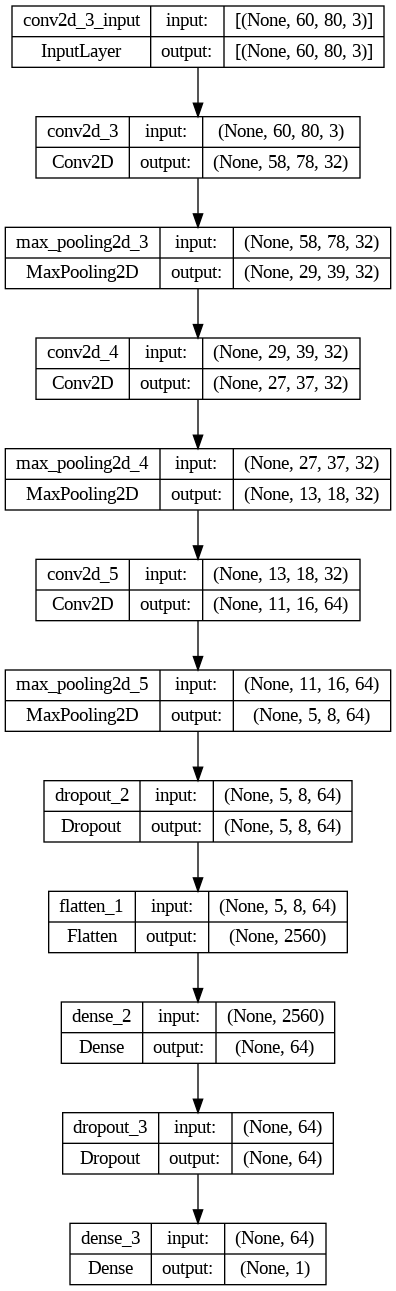
\includegraphics[width=.5\columnwidth]{cnn2}
    \caption{Struktura konwolucyjnej sieci neuronowej wykorzystanej do sterowania robotem Duckiebot.}
    \label{fig:cnn-structure}
\end{figure}

Sieć składa się z pierwszej warstwy konwolucyjnej, następną warstwa jest warstwa \emph{MaxPooling}. Jej zdaniem jest zredukowanie rozmiaru danych wejściowych. Kolejne  warstwy sieci to warstwa konwolucyjnej i warstwa MaxPooling - taki układ warstw jest powtórzony dwukrotnie. Za każdym razem warstwy konwolucyjne ekstrahują kolejne cechy obrazu wejściowego istotnie z punktu wiedzenia sterowania robotem Duckiebot, natomiast warstwy \emph{MaxPooling} redukują rozmiar danych. Zadaniem następnej warstwy \emph{Dropout} losowe wyłączanie poszczególnych neuronów sieci, tak aby zapobiec zjawisku \emph{overfitting} oraz wspomóc zdolność generalizacji sieci neuronowej. Przed przesłaniem danych na wejście właściwej sieci neuronowej muszą one zostać spłaszczone co jest zadaniem warstwy \emph{Flatten}. Przekształca ona dane wielowymiarowe w jednowymiarowy wektor wejściowy do następnej warstwy \emph{Dense}. Warstwa \emph{Dense} jest jest odpowiedzialna za wykonywanie klasyfikacji, regresji lub innych zadań uczenia maszynowego. Wyjściem z sieci CNN jest wartość sygnału $\omega$ z przedziału $[-8\: ; \:8]$ dlatego funkcją aktywacji jest z wyjścia warstwy \emph{Dense} jest funkcja \emph{tanh}.

\subsection{Przygotowanie danych}
Każda sieć neuronowa jest tak dobra jak dobrymi danymi została wytrenowana. Stąd też bardzo ważnym etap pracy z sieciami neuronowymi jest przygotowanie dobrego zbioru danych uczących. W przypadku robota Duckiebot i zadania które ma realizować (\emph{line follower}) dane uczące dla sieci składają się z par: obraz z kamery i odpowiadająca mu prawidłowa wartość $\omega$, zob. rys. \ref{fig:cnn-pipeline}. Dane konieczne do trenowania sieci można uzyskać sterując robotem Duckiebot ręcznie (np. za pomocą gamepad) lub wykorzystać opracowany wcześniej układ sterowania z regulatorem PID dodając skrypt zapisujący dane. 

Oprócz odpowiedniej ilości zalogowany danych do uczenia sieci neuronowej, ważne jest aby dane te były odpowiednio różnorodne - czyli aby obejmowały jak największą liczbę przypadków, sytuacji, zdarzeń w jakich może znaleźć się robot Duckiebot. Na rysunku \ref{fig:cnn-data-hist1} przedstawiono histogram przykładowego zbioru danych jaki został zalogowany. 

\begin{figure}[h]
	\begin{subfigure}{.475\columnwidth}
    	\centering
    	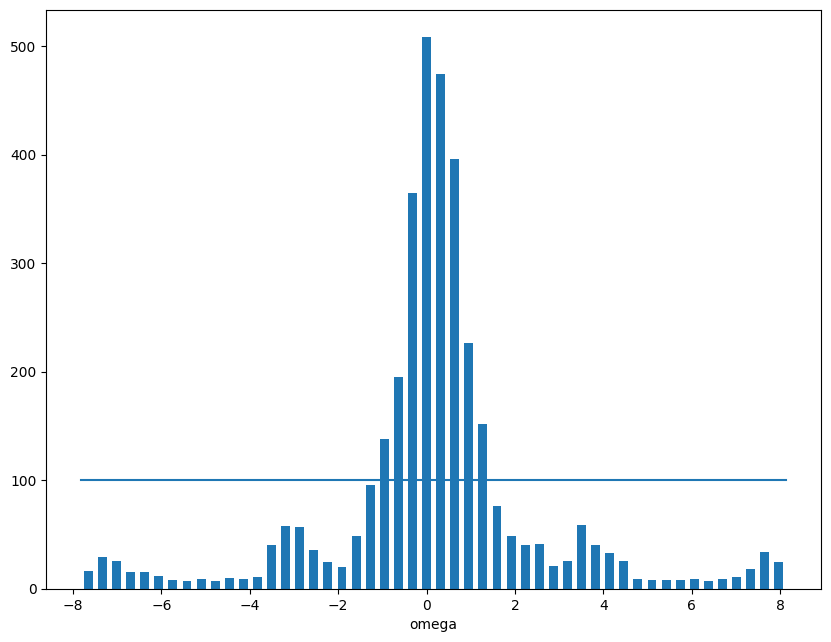
\includegraphics[width=1\columnwidth]{h1}
    	\caption{}
    	\label{fig:cnn-data-hist1}
    \end{subfigure}
    \begin{subfigure}{.475\columnwidth}
    	\centering
    	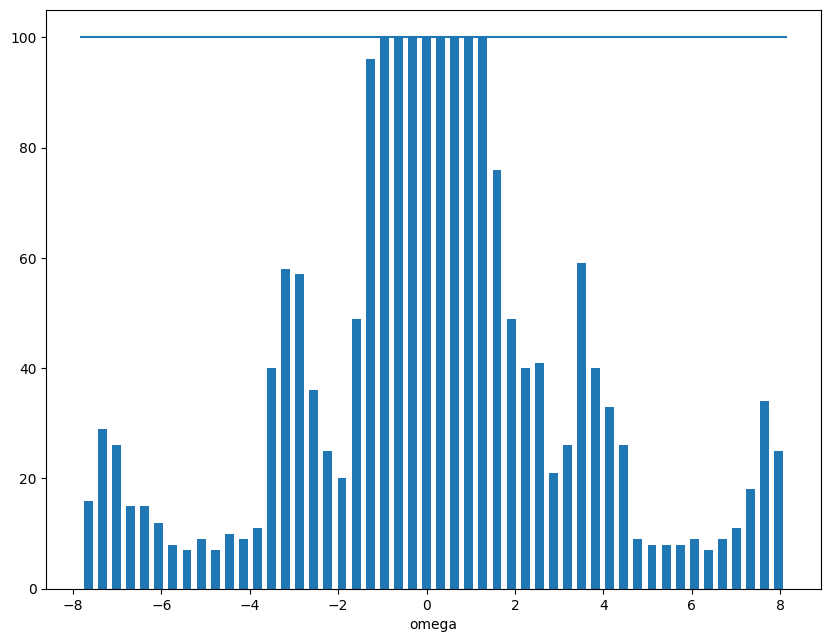
\includegraphics[width=1\columnwidth]{h2}
    	\caption{}
    	\label{fig:cnn-data-hist2}
    \end{subfigure}
    
    \caption{Histogram zalogowanych danych przed analizą a) i po analizie b).}
    \label{fig:cnn-data-hist}
\end{figure}

Wyraźnie widać, że dominującą wartością w tym zbiorze danych dla zmiennej $\omega$ są wartości w bliskie wartości $0$ i jeśli użyć takich danych do trenowania sieci CNN która ma sterować robotem Duckiebot to prawdopodobnie robot bardzo dobrze jeździł by prosto, natomiast miał by problemy z zakrętami. W takim przypadku, po analizie danych należy usunąć ze zbioru uczącego dane których wartości znacząco dominują nad innymi wartościami otrzymując bardziej reprezentatywny zbiór danych uczących, zob. rys. \ref{fig:cnn-data-hist2}.

Podobnie jak w przypadku sterowania robotem Duckiebot z wykorzystaniem regulatora PID tak i w przypadku sterowania robotem Duckiebot z wykorzystaniem sieci neuronowych konieczne jest odpowiednie przygotowania obrazów z kamery. Poszczególne etapy przetwarzania obrazów z kamer robota Duckiebot przedstawiono na rysunku \ref{fig:cnn-pipeline} (bloki o kolorze żółtym) i są to: przycinanie obrazu do interesującego nas obszaru, konwersja do przestrzeni barw YUV (Y-luminacja, UV-barwa kolorów, chrominancja), filtrowanie z wykorzystaniem filtru Gauus-a, zmiana rozmiaru obrazu i normalizacja wartości poszczególnych kanałów obraz do przedziału $[0\;1]$. Rezultat poszczególnych operacji można zobaczyć na rysunku \ref{fig:cnn-image-prepare}.

\begin{figure}[h]
    \centering
    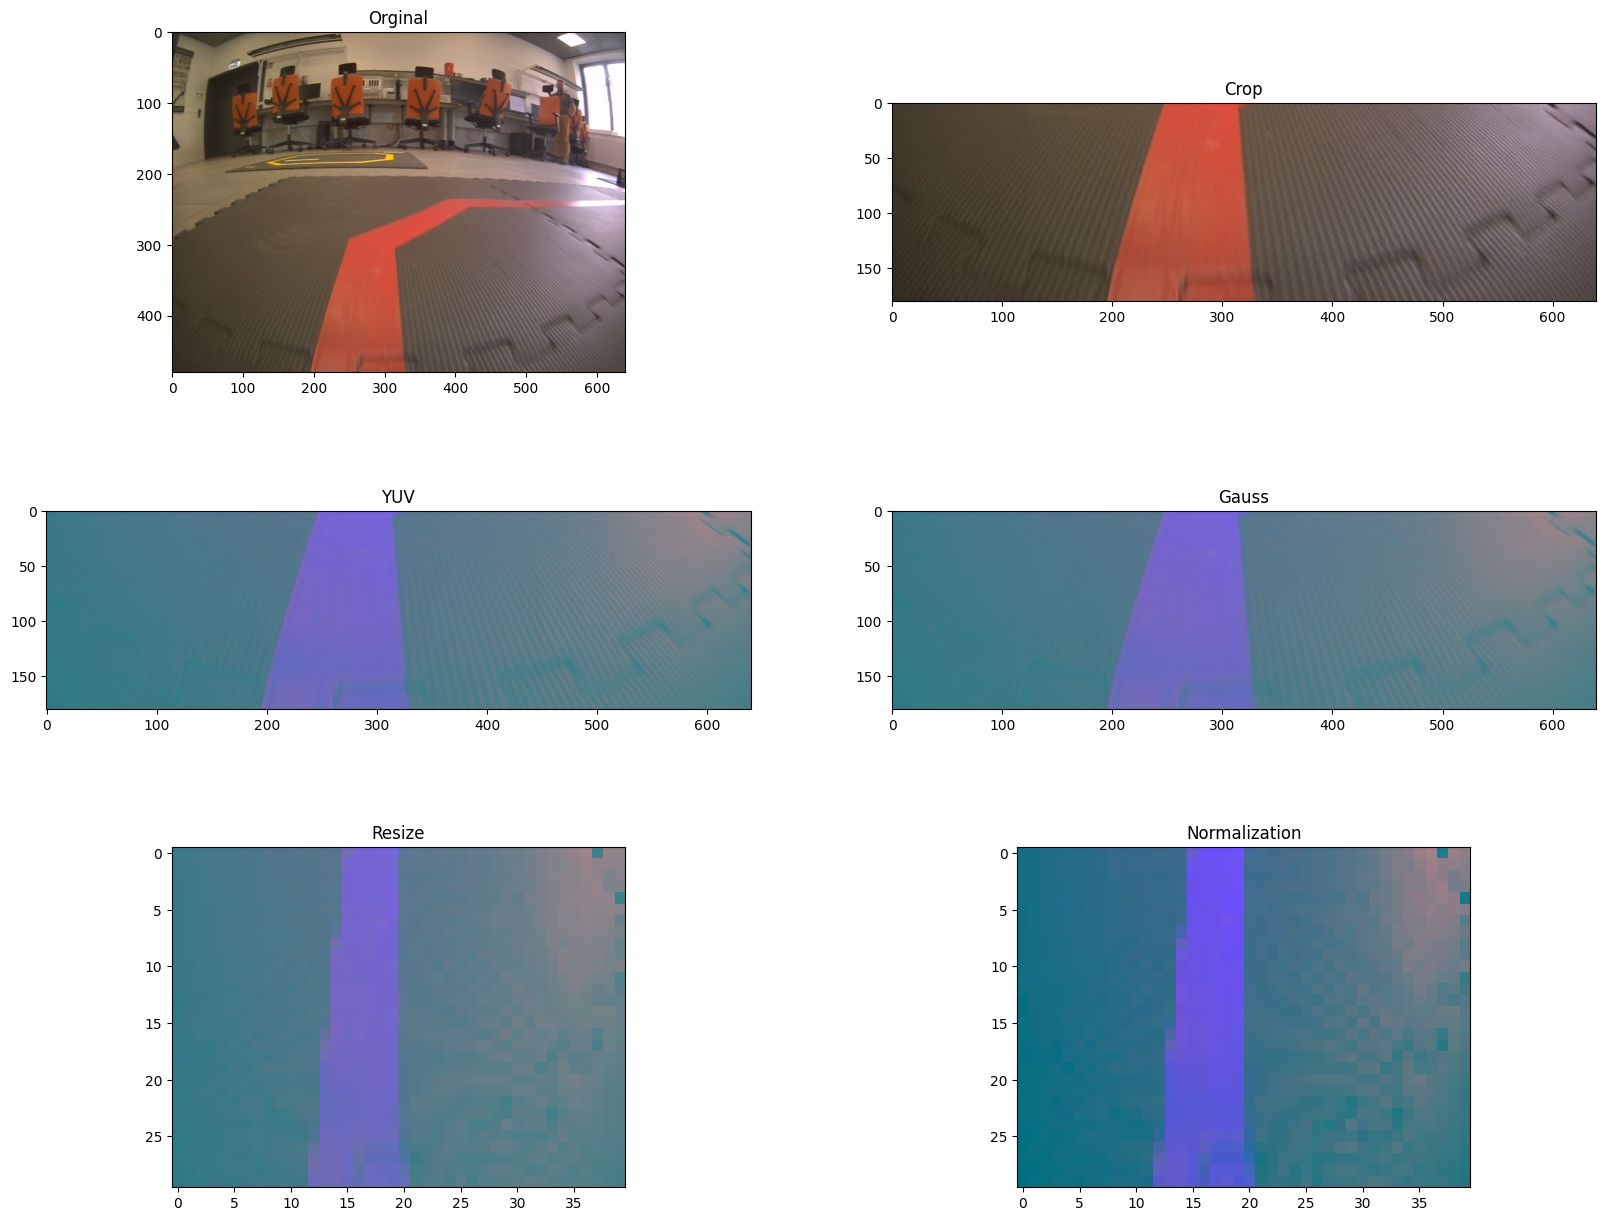
\includegraphics[width=.95\columnwidth]{nn_prepare_image}
    \caption{Operacje wykonywane na obrazach z kamery robota Duckiebot sterowanym przed zastosowanie regulatora CNN.}
    \label{fig:cnn-image-prepare}
\end{figure}

%%%%%%%%%%%%%%%%%%%%%%%%%%%%%%%%%%%%%%%%%%%%%%%%%%%%

\section{Praktyczne wskazówki}\label{sec:practical-info}
Oprogramowanie robotów Duckietown zostało zaimplementowane z wykorzystaniem framework-a Robot Opertion System (\emph{ROS}) \cite{quigley2015programming}. Jest on obecnie jednym z najpopularniejszym framework-ów do programowania rożnego rodzaju robotów. Konsekwencją wybrania framework-a ROS jest wybór języka programowania i w przypadku robotów Duckiebot jest to Python. Projekt Duckietown definiuje również sposób tworzenia własnego oprogramowania dla robotów i wymusza stosowanie technologi konteneryzacji. Jest to bardzo dobra praktyka zgodna z ówczesnymi trendami tworzenia oprogramowania. Dokładny opis w raz z przykładami tworzenia oprogramowania dla robotów Duckie jest bardzo dobrze opisany w dokumentacji projektu \cite{Daniele:ff}. 
Wykorzystanie framework-a ROS umożliwia również efektywnie tworzenie i testowania oprogramowania bez konieczności ciągłego wygrywania kolejnych wersji do robota Duckiebot. Konfigurując odpowiednio komputer host-a, tak aby łączy się z serwerem ROS-na uruchomionym na wybranym robocie Duckiebot można w sposób wygodny i efektywny implementować i testować własne oprogramowanie, zob. rys. \ref{fig:env-develop}.

\begin{figure}[h]
    \centering
    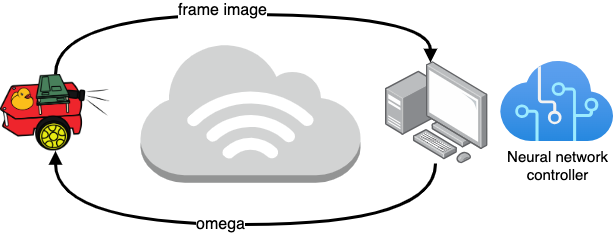
\includegraphics[width=.8\columnwidth]{controll_schema2}
    \caption{Konfiguracja środowiska deweloperskiego dla robota Duckiebot.}
    \label{fig:env-develop}
\end{figure}

Proponowane regulatory należy zaimplementować jako węzły ROS-a. Węzły powinny odczytywać obrazy z kamery robota (przesyłane jako wiadomości ROS) a jako wyjście generować sygnał sterowania $\omega$. Dla uproszczenia sterowania robotem Duckiebot można przyjąć, że porusza się on ze stała prędkością liniową $v=const$.

Konwolucyjne sieci neuronowe można tworzyć, trenować oraz testować wykorzystując moduły \emph{keras} i \emph{tensorflow} języka Python. Zaletą modułów \emph{keras} i \emph{tensorflow} jest również bardzo dobra dokumentacja z bardzo duża ilością przykładów. 

Należy zwrócić również uwagę prawidłowe przygotowanie danych do uczenia sieci neuronowych, każdemu obrazowi z kamery musi odpowiadać jedna, poprawna wartość sygnału $\omega$.

%%%%%%%%%%%%%%%%%%%%%%%%%%%%%%%%%%%%%%%%%%%%%%%%%%%%

\section{Wnioski}\label{sec:conclusion}
Regulator PID jest stosowany z powodzeniem w wielu układach sterowania a jego implementacja jest stosunkowo prosta. Dla tego typu regulatorów istnieje również szereg metod i algorytmów doboru parametrów regulatora. Regulatory PID nie są wolne też od wad. Jedną z nich jest znajomość, choćby przybliżonego, modelu procesu jakim chcemy sterować. Zachodzi więc konieczność identyfikacji zarówno struktury modelu procesu jak i jego parametrów. Zadania identyfikacji nie są zadaniami prostymi, wymagają dużej wiedzy odnośnie istoty samego procesu. Istnieją również metody identyfikacji modelów procesów bazujące na wynikach eksperymentów praktycznych, ale w tym przypadku może się okazać, że przeprowadzanie takiego eksperymentu nie zawsze jest możliwie. Stosują regulator PID należy również mieć świadomość, że został on opracowany dla procesów których działanie można opisać modelami liniowymi. Niestety, działanie zdecydowanej większości systemów dynamicznych jest opisane modelami nieliniowymi. Konsekwencją tego jest fakt, że w takim przypadku regulator PID działa wykorzystując liniowe przybliżenia systemów nieliniowych - co może być przyczyną różnych błędów, niedokładności itp.

W przeciwieństwie do klasycznego regulatora PID, regulatory wykorzystujące sztuczne sieci neuronowe nie potrzebują znajomości modelu matematycznego procesu którym sterują oraz jego parametrów. Możliwość projektowania różnych architektur sieci neuronowych, takich jak konwolucyjne, rekurencyjne czy głębokie sieci neuronowe, umożliwia dostosowanie regulatora neuronowego do konkretnego procesu którym mają sterować. Z drugiej strony, mnogość architektur sieci neuronowych, ich budowa powoduje, że nigdy nie mamy pewności czy dana struktura sieci neurnowej jest optymalna.
Dobór parametrów regulatorów neuronowych odbywa się w sposób automatyczny poprzez wykorzystanie odpowiednich algorytmów uczenia sieci.  Kluczowym elementem mającym wpływ na poprawność pracy regulatora neuronowego są dane jakim jest uczona sieć neuronowa. Wadą regulatorów wykorzystujących sieci neuronowe jest brak możliwości wykazania stabilności działania układów którymi sterują. W przypadku regulatora PID, pomimo wykorzystywania przybliżonych modeli procesu bardzo często można udowodnić, że zamknięty układ sterowania będzie pracował stabilnie w każdych lub w pewnym zakresie wartości zmiennych. Niestety takiej analizy nie da się przeprowadzić w przypadku regulatorów neuronowych. 

Podsumowując implementacja dwóch różnych regulatorów do realizacji tego samego zadnia daje możliwość poznania zalet i wad każdego z nich. Studenci w trakcie rozwiązywania postawionego problemu muszą wykazać się znajmością teoretyczną  zagadnień oraz, co jest szczególnie istotne w przypadku inżynierów, nabywają umiejętności praktycznego stosowania wiedzy teoretycznej. 


\bibliographystyle{IEEEtran}
\bibliography{references}

\end{document}
